\chapter{Personalplaner}\label{personal:mitglieder}
Im Kopf des Fensters aus \cref{fig:personal:mitglieder} kann eingestellt werden welche Personen angezeigt werden sollen.
Ebenso kann durch einen Knopfdruck eine E-Mail an alle angezeigten Personen erstellt werden.
Werden bei dieser Aktion Personen gefunden, für die keine Mailadresse angegeben ist,
so können die hinterlegten Postadressen in einer CSV-Datei gespeichert werden.
Diese Daten können dann z.B.\ für Serienbriefe genutzt werden.


\begin{figure}[!h]
	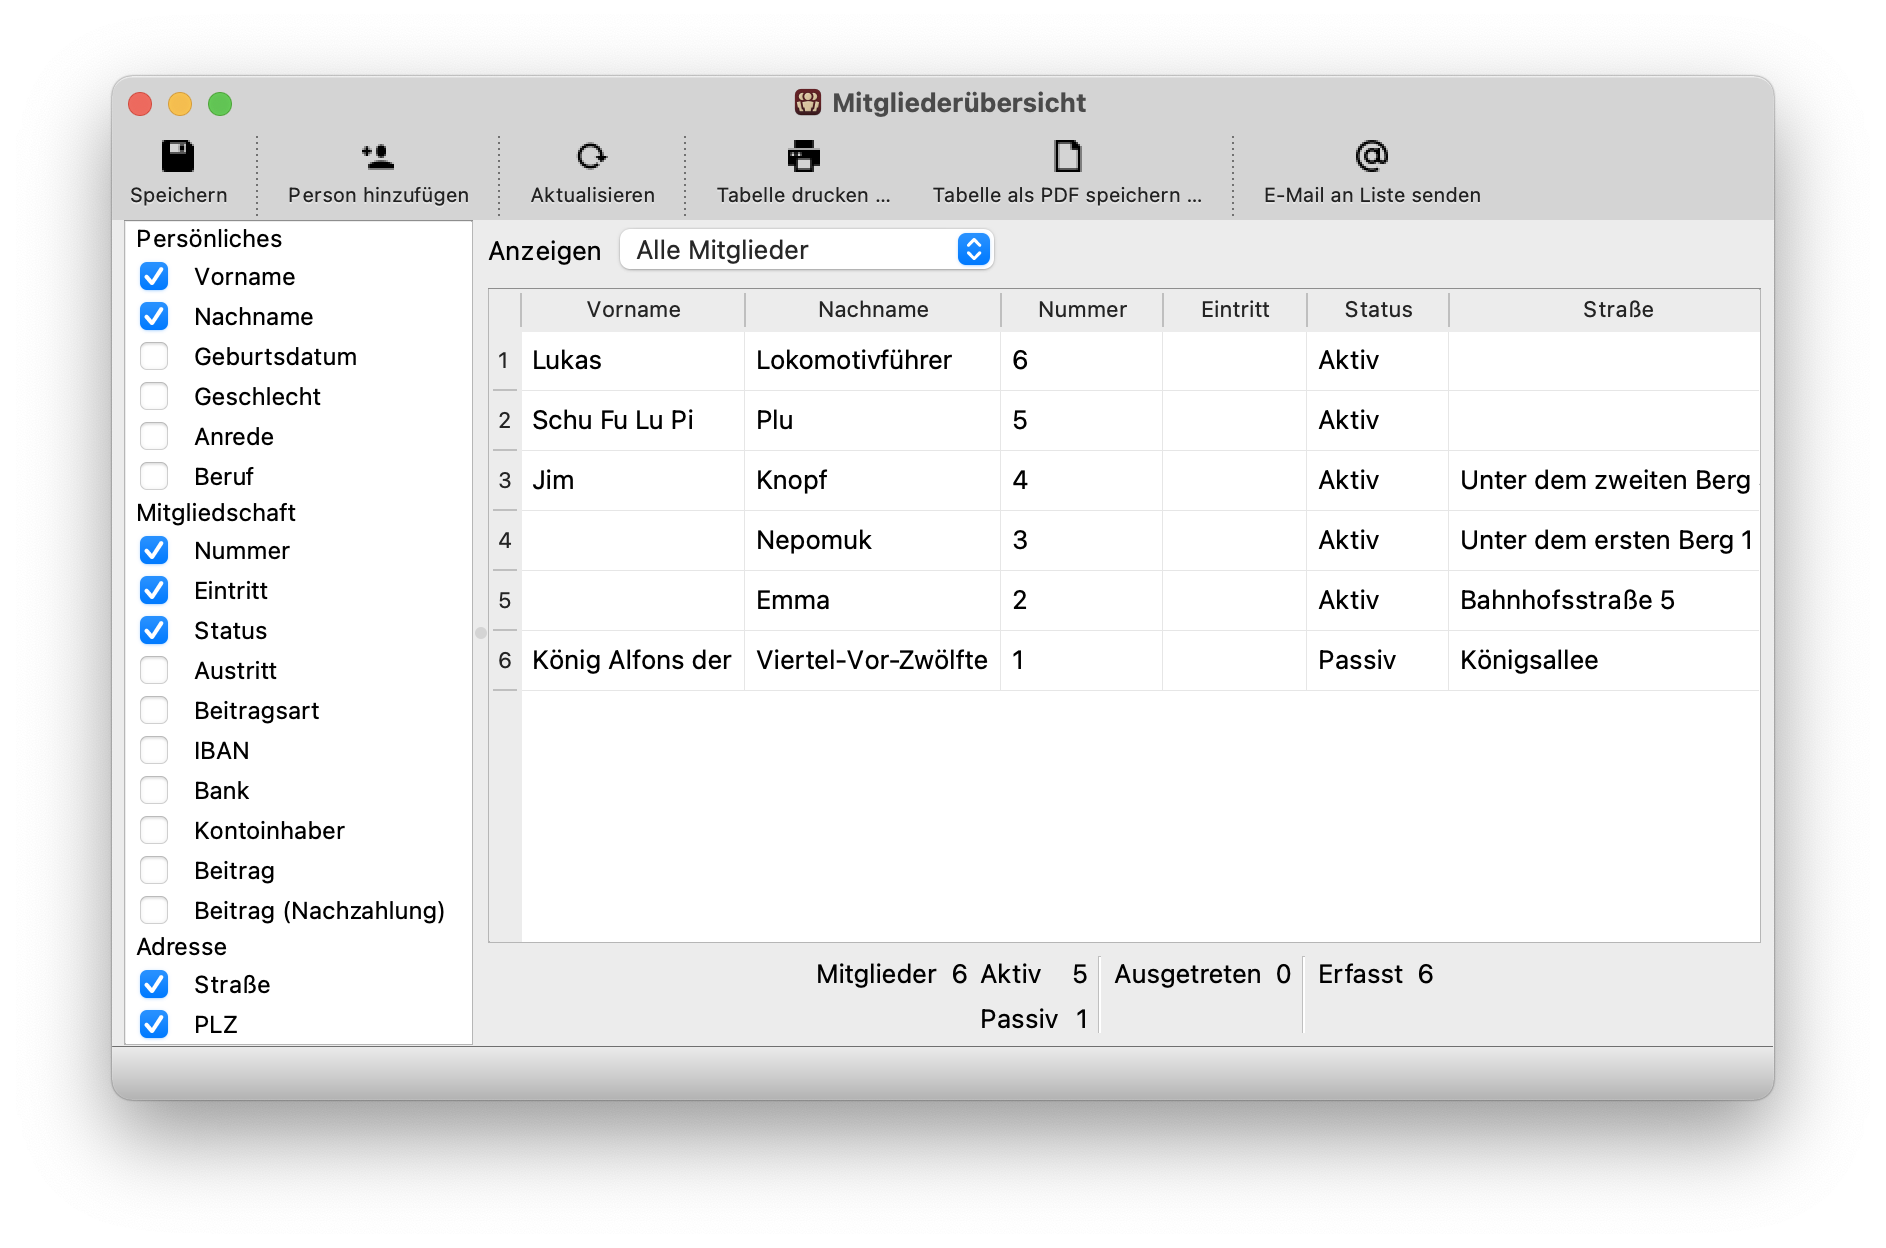
\includegraphics[width=\textwidth]{img/personal-liste}
	\caption{Die Mitgliederliste mit allen ausgewählten Mitgliedern.}
	\label{fig:personal:mitglieder}
\end{figure}

Die Einzelansicht einer Person kann über einen Doppelklick auf eine Zelle der entsprechenden Zeile geöffnet werden.

Über eine ent- bzw.\ zusammenfaltbare Liste auf der linken Seite des Fensters kann eingestellt werden,
welche Daten in der Tabelle angezeigt werden.
Im unteren Bereich des Fensters wird eine kurze Statistik
der aktuellen und ausgetretenen Mitglieder angezeigt.

\paragraph{Export}
Die Tabelle kann über die Knöpfe \button{Tabelle drucken} und \button{Tabelle als PDF speichern} ausgegeben werden.
Über das Menü \aktion{Exportieren} steht noch ein Export als CSV-Datei zur Verfügung (hier werden alle gespeicherten Daten exportiert),
sodass die Daten in anderen Programmen verarbeitet werden können.
Ebenso besteht die Möglichkeit über den Eintrag \aktion{Stammdatenblätter} die Daten eines Mitglieds bzw.\ aller angezeigten Personen auszugeben.
Hierbei wird für jede Person eine Seite erzeugt, die in einem gemeinsamen Dokument gespeichert werden.


\begin{neu}
\section{Mitgliedsbeiträge}\label{personal:mitglieder:beitrag}
Über das Menü \aktion{Bearbeiten} können Sie unter \aktion{Mitgliedsbeiträge} einen Dialog aufrufen,
in dem die Höhe der Mitgliedsbeiträge festgelegt werden kann.
Siehe \cref{fig:personal:mitglieder:beitrag} für ein Beispiel.

\begin{figure}[!h]
  \centering
	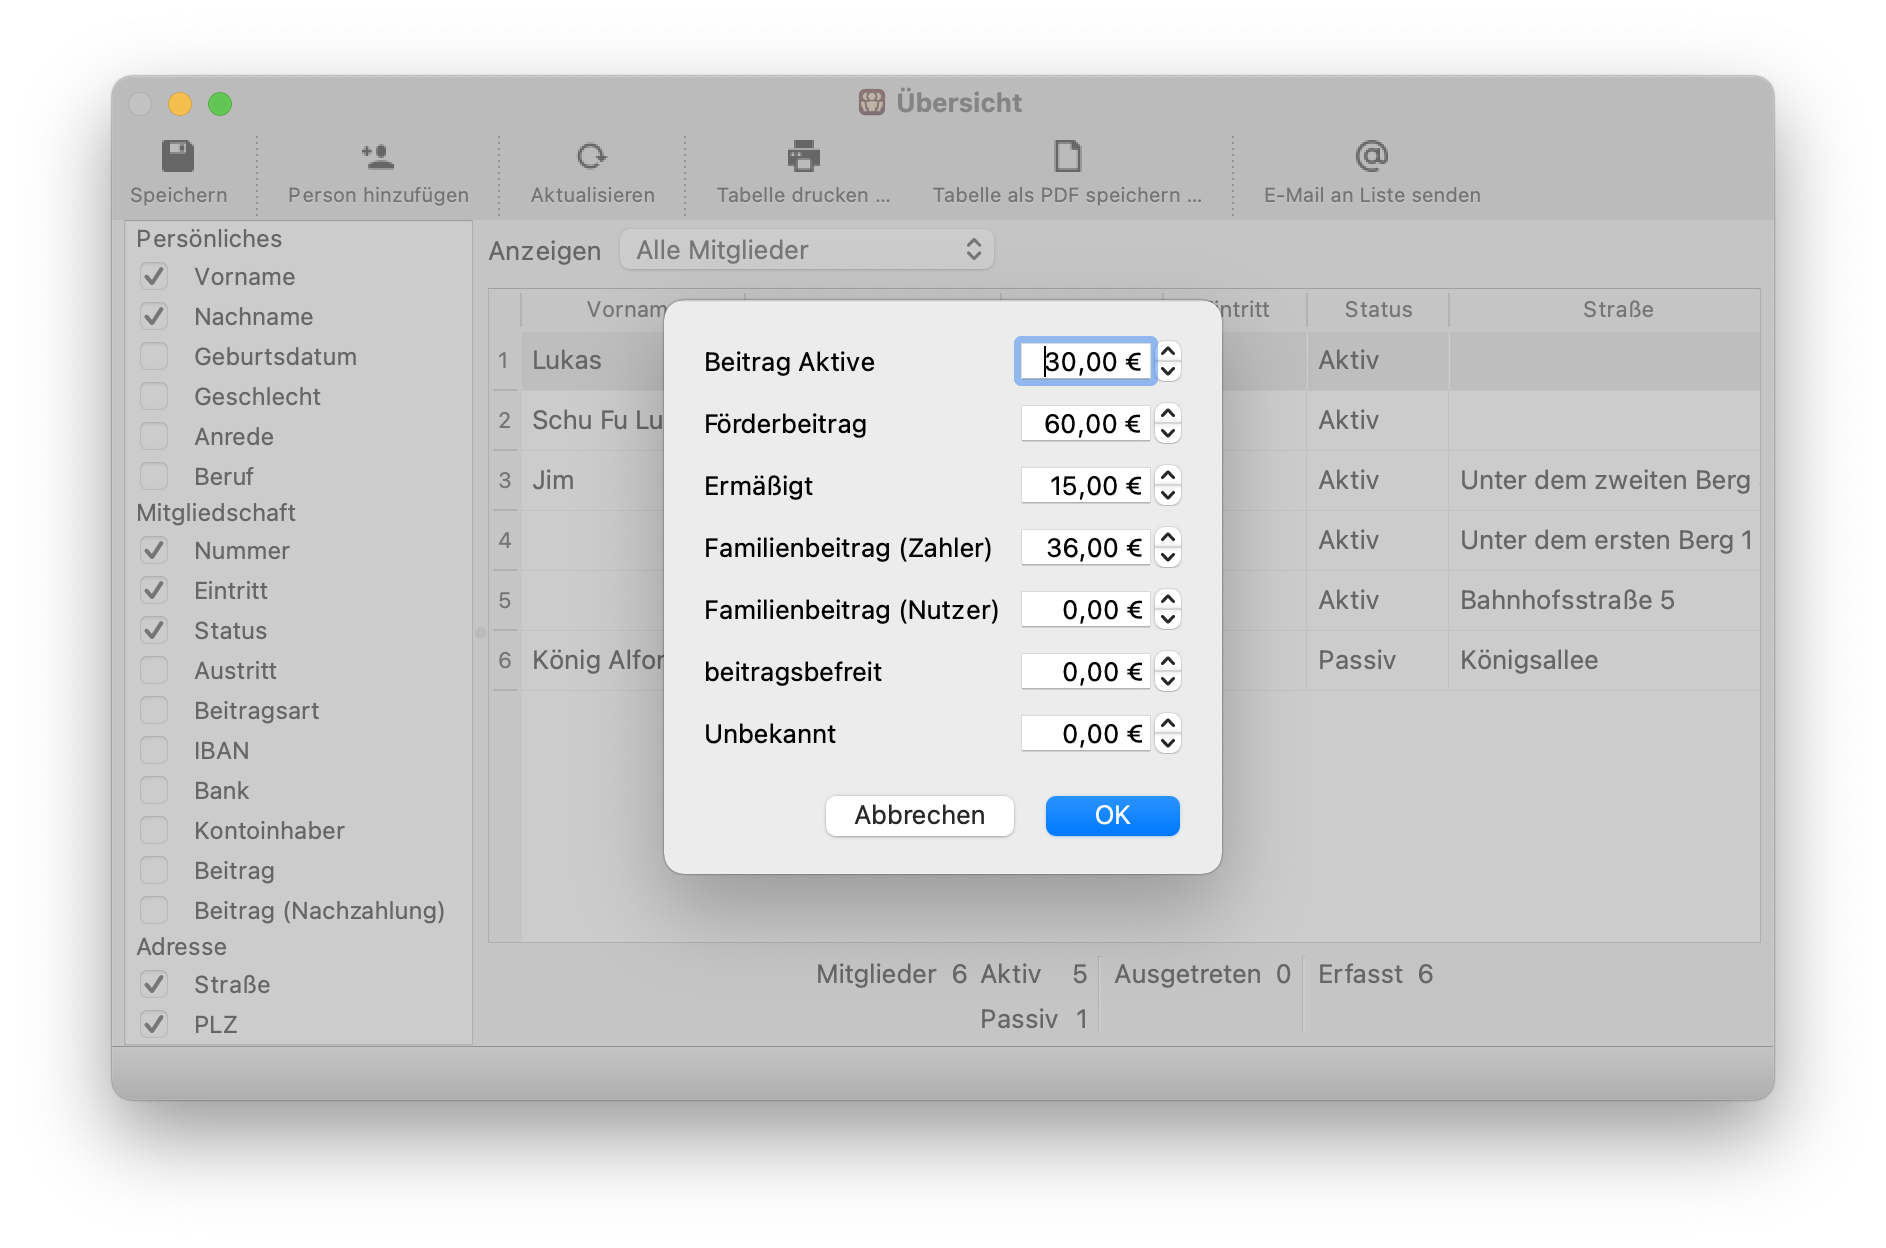
\includegraphics[width=0.75\textwidth]{img/personal-beitrag}
	\caption{Der Dialog zum Festlegen der Höhe der Mitgliedsbeiträge.}
	\label{fig:personal:mitglieder:beitrag}
\end{figure}

Bei den Beiträgen wird zwischen zwei verschiedenen Arten unterschieden.
Der reguläre Beitrag umfasst den Jahresbeitrag basierend auf der Mitgliedschaft der Personen, z.B.\ Aktive Mitglieder, Ermäßigte, \dots.
Dieser Beitrag kann im Dialog eingestellt werden.
Die zweite Art umfasst die Nachzahlungen.
Da aktive Vereinsmitglieder Pflichtstunden erbringen müssen,
erhöht sich ihr Beitrag wenn dies nicht geschieht.
Dieser Beitrag wird automatisch aufgrund der vorliegenden Daten des \Einsatz berechnet.
Mitglieder die ihre Pflichtstunden nicht erfüllt haben, müssen einen zusätzlichen Beitrag bezahlen, der sich nach der Anzahl der erbrachten Stunden richtet.

Im ersten Schritt wird der individuelle reguläre Beitrag ermittelt.
Dies entspricht im Allgemeinem dem eingestellten Beitrag.
Bei einem Familienbeitrag wird der Beitrag gleichmäßig auf alle Mitglieder umgelegt,
die Pflichtstunden zu erbringen haben.
Danach wird der Prozentsatz der nicht erbrachten Stunden berechnet
(1 - erbrachte Stunden / erforderliche Stunden).
Dieser Prozentsatz ergibt multipliziert mit der Differenz aus Förderbeitrag und individuellem regulärem Beitrag die Höhe der Nachzahlung.
Somit erhöht sich der Beitrag durch die Nachzahlungen bis auf den Förderbeitrag.


Für den Beitragseinzug können beide Arten von Beiträgen ausgegeben werden.
Dazu stehen im Menü \aktion{Export} die beiden Funktionen \aktion{Export Jahresbeiträge \dots} und \aktion{Export Nachzahlungen \dots} zur Verfügung.
Über diese Wird jeweils eine CSV-Datei erstellt, die folgende Informationen enthält:
\begin{itemize}
  \item
  Name des Mitglieds und Mitgliedsnummer
  \item
  Höhe des Beitrags (je nach ausgewählter Art)
  \item
  Daten der Bankverbindung (IBAN, Bank, Kontoinhaber).
  Bei einer Familienmitgliedschaft werden die Daten des Zahlers für die Bankverbindung übernommen.
  Das Eintragen von Daten für den Nutzer ist nicht erforderlich,
  vielmehr werden diese Daten beim Export über die Beitragsfunktion ignoriert.
\end{itemize}

Die Beiträge können auch über die Tabelle angezeigt und ausgegeben werden,
indem die entsprechenden Spalten in der Tabelle angezeigt werden.
\end{neu}
